\documentclass[a4paper]{report}
\usepackage{algorithmic}
\usepackage{array}
\usepackage{url,amsfonts,amsmath,amssymb,amsthm,color,enumerate,tikz,hyperref}
\usepackage{algorithm,bbm}
\usepackage{mathtools}
% \usepackage{indentfirst}
\usepackage{stackrel}
\usepackage{listings}
\usepackage{subfigure}
\usepackage{subfloat}
\usepackage[justification=centering]{caption}
\usepackage{booktabs} % for three-line table
% \usepackage{subfig}
\usepackage{graphicx}
\setcounter{tocdepth}{4}
\setcounter{secnumdepth}{4}

\hyphenation{op-tical net-works semi-conduc-tor}
\usetikzlibrary{shapes, shadows, arrows}
% \usepackage[english]{babel}
% \usepackage[utf8]{inputenc}
% \usepackage{amsmath}
% \usepackage{graphicx}
% \usepackage[colorinlistoftodos]{todonotes}

\title{Get Start with gr-cdma}

\author{Yu Wang\\umwangyu@umich.edu}

\date{\today}

% def some function
\DeclarePairedDelimiter\ceil{\lceil}{\rceil}
\DeclarePairedDelimiter\floor{\lfloor}{\rfloor}

\begin{document}
\maketitle
\tableofcontents
\newpage




\chapter{Introduction}
\section{What is gr-cdma}
Project gr-cdma is the physical layer of CDMA communication. This project is developed based on GNURadio\cite{GNURadio}.
gr-cdma is created and maintained by Prof. Anastasopoulos.
The whole source codes are on github \url{https://github.com/anastas/gr-cdma}.
This project is to build a communication block which employs DS-CDMA technique to build the link.
The user does not have to know the details of the schemes, but could transmit reliably through this physical layer protocol.

\section{What is GNURadio}
GNURadio\cite{GNURadio} is a open-source *unix based platform which enables developers and researchers design and test their self-built communication or signal processing system.
The whole platform is written by c++. Developer could use c++ or python to customize their own block. gr-cdma is a customized block as well.

\section{What is the Current State of gr-cdma}
Till 17-Jun-2016, the main part of this project is finished.
The next step is to optimize the working strategy for several block to make the system more robust in field test. 
This document is an introduction of what this project is, how to get start with GNURadio and gr-cdma and what are the issues to be solved. 
\chapter{Working Strategy of gr-cdma}
In this chapter, we will discuss the working strategy of gr-cdma, the principle of each main block.
Mathematic models and analyses are involved to describe the situation.

\section{The diagram of The Tx \& Rx}
Here are the digrams for Tx and Rx. 
\begin{figure}[!ht]
	\centering
	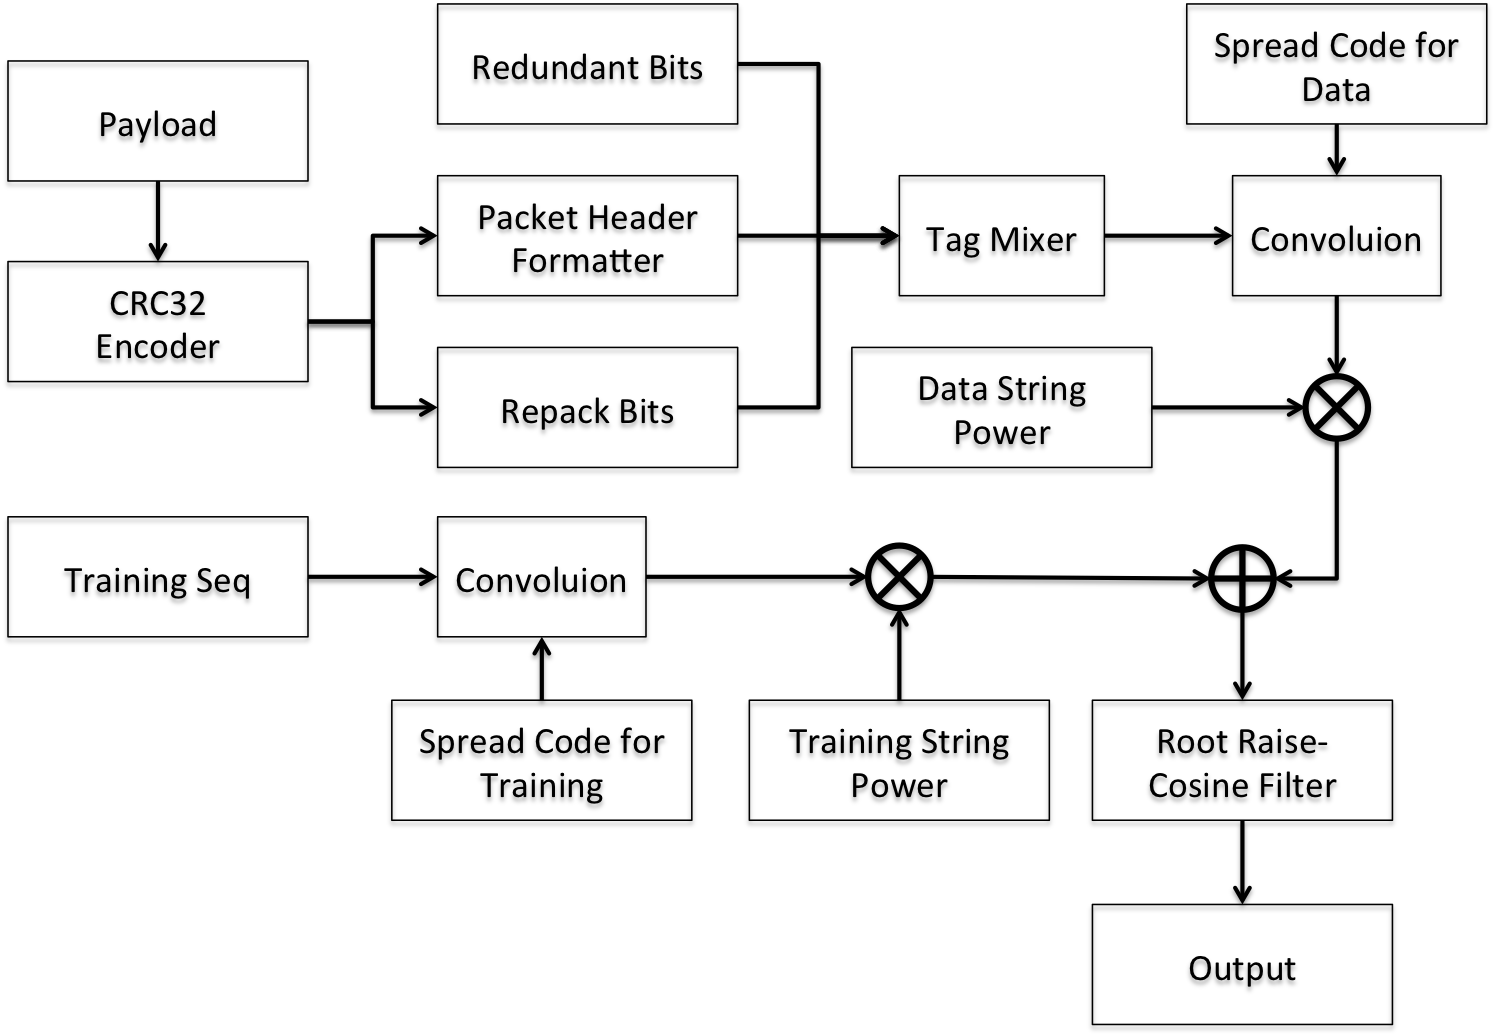
\includegraphics[width = 5 in]{figure/tx-diagram.png}
	\caption{Diagram for Tx}
	\label{fig:diagram for Tx}
\end{figure}
\begin{figure}[!ht]
	\centering
	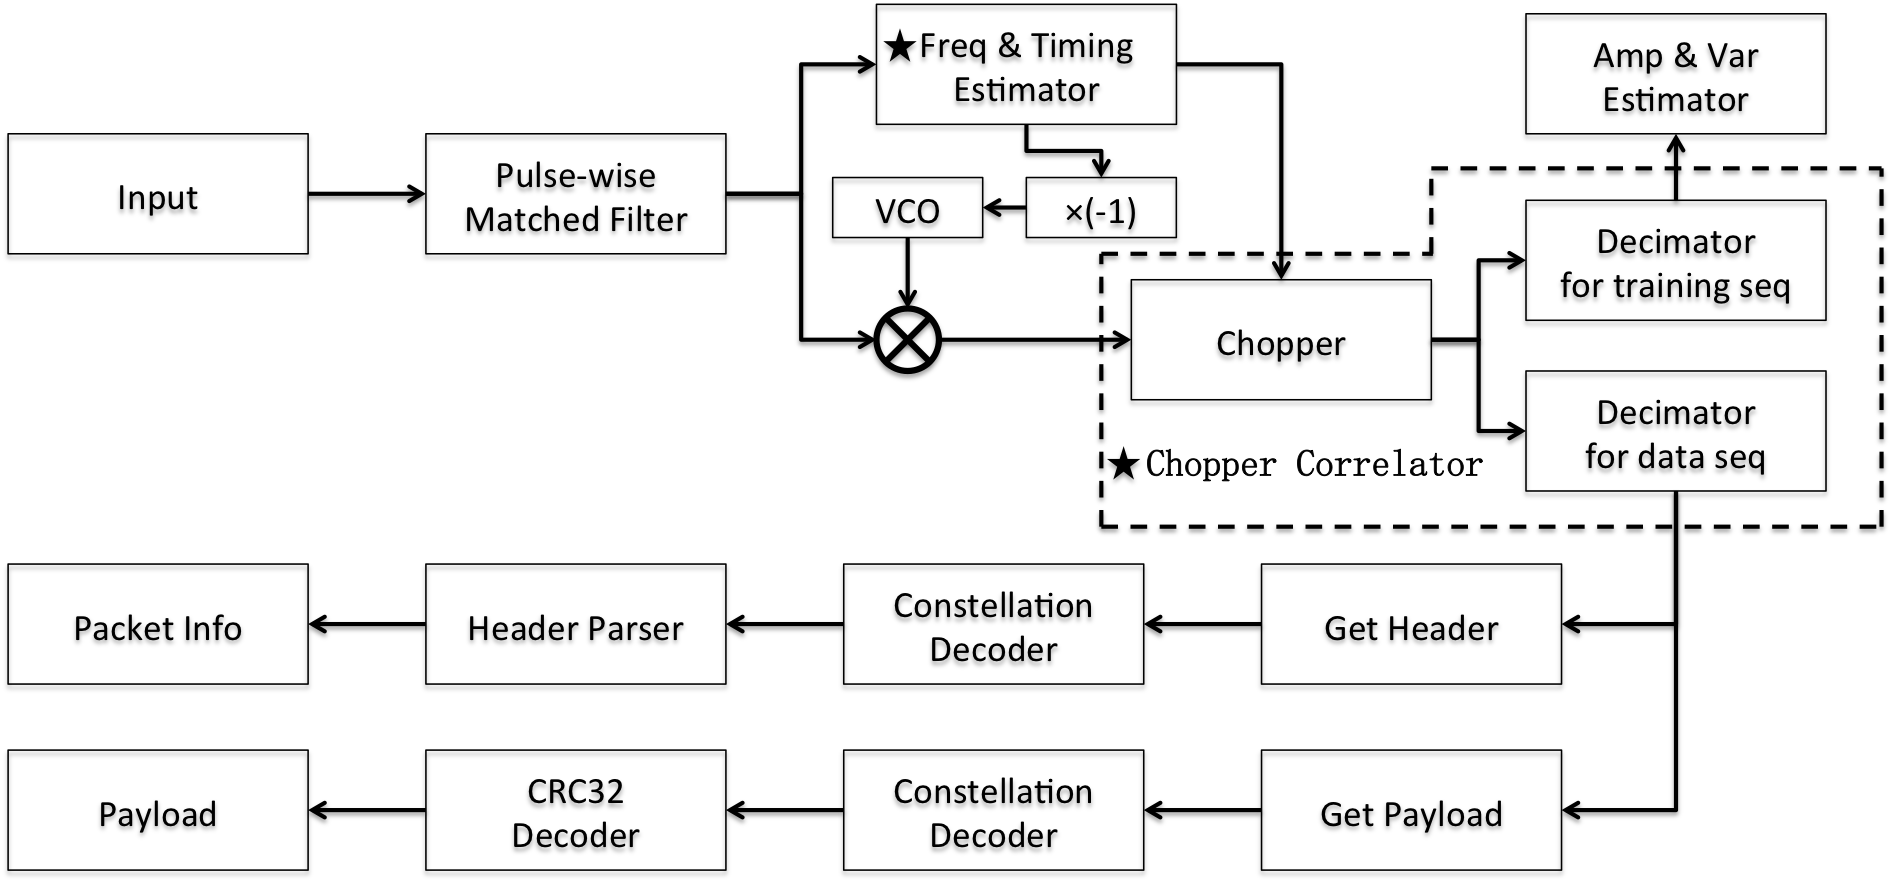
\includegraphics[width = 5in]{figure/rx-diagram.png}
	\caption{Diagram for Rx}
	\label{fig:diagram for Rx}
\end{figure}

From fig \ref{fig:diagram for Tx} and fig \ref{fig:diagram for Rx}, you may find that the system is a little bit more complicated than you thought. And also, the receiver is bigger than the transmitter. In fact, it is for the reason that the receiver will deal with no only the decoding part, but also the synchronization problem. which is actually the most difficult part for this system.

\section{Transmitter} % (fold)
\label{sec:transmitter}
The duty for transmitter is to package the payload or the input data, build the packet structure, generate the training sequence, modify the power for each section and form the waveform. Similar to other CDMA system, one of the essential part of the system is about the spreading code. The quality of the spreading code will affect greatly about the performance of synchronization parts. Intuitively, we would like to use codes like m-sequences and gold sequence, which has high auto-correlation and flat cross-correlation value.

\begin{figure}
	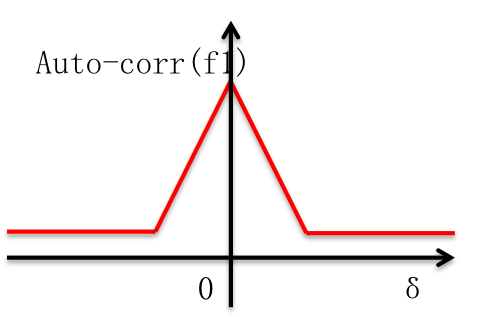
\includegraphics[width = 3in]{figure/bad_correlation.png}
	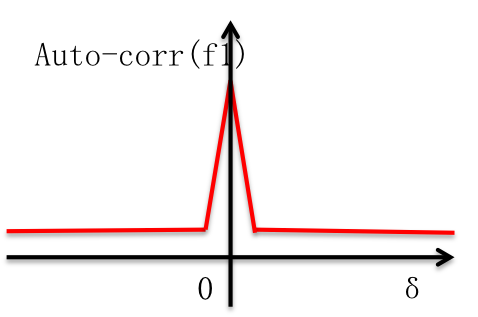
\includegraphics[width = 3in]{figure/good_correlation.png}
\end{figure}

% section transmitter (end)



\bibliographystyle{plain}
\bibliography{bibliography.bib}

\end{document}
